% Modified: 07-17_22-35
% Changes: ResearchPilot G.7 reframed IHP as a coordinate-contract audit and
% minimal repair, prioritized same-cache evidence, and disclosed protocol and
% post-selection limits. Previous version remains available in Git history.
%
% === PAPER ARCHITECTURE ===
% Title: Auditing and Repairing Multiscale Coordinate Projection in Frozen
%        Visual Time-Series Anomaly Detection
% Target: IEEE MSN 2026 Regular Paper, Big Data and AI, anonymous English
% Format: IEEE conference, US Letter, 10 pt, two columns, <= 8 pages
%
% I. Introduction
%   Problem and telemetry relevance; coordinate-contract failure; IHP preview;
%   three evidence-mapped contributions. Place Fig. 1 after method preview.
% II. Related Work
%   Numerical/foundation-model TSAD; visual/multimodal TSAD; structured visual
%   localization and coordinate-aware aggregation.
% III. Index-Consistent Harmonic Projection
%   A. Frozen visual screening and notation.
%   B. Failure mechanism: shifted support graph.
%   C. Literal incidence repair; complete-coverage property.
%   D. Inherited harmonic projection on corrected support.
%   E. Frozen-system integration, invariants, and complexity.
% IV. Experimental Protocol
%   Data, external/local comparator boundary, metrics, uncertainty, environment.
% V. Results and Analysis
%   A. Complete 11-subdataset paper-reported comparison (Table I).
%   B. Same-cache component ablation and paired CIs (Table II).
%   C. Structural/system analysis (Table III and Fig. 2).
% VI. Limitations and Conclusion
%   Bounded claims, untested scope, and mechanism-to-system takeaway.
% === END PAPER ARCHITECTURE ===

\documentclass[conference]{IEEEtran}

\usepackage{cite}
\usepackage{amsmath,amssymb,amsfonts}
\usepackage{booktabs}
\usepackage{graphicx}
\usepackage{textcomp}
\usepackage{url}

\begin{document}

\title{Auditing and Repairing Multiscale Coordinate Projection in Frozen Visual Time-Series Anomaly Detection}

\author{\IEEEauthorblockN{Anonymous Authors}}

\maketitle

\begin{abstract}
This provisional source verifies the anonymous IEEE conference layout only.
The final abstract, numerical results, and contribution claims are intentionally
withheld until the frozen Phase F benchmark and claim--evidence gate complete.

\end{abstract}

\begin{IEEEkeywords}
time-series anomaly detection, telemetry monitoring, visual foundation models,
coordinate consistency, harmonic projection
\end{IEEEkeywords}

\section{Introduction}

Telemetry anomaly detection must distinguish rare operational incidents from
normal temporal variation without allowing test labels to shape the detector.
This provisional section reserves the publication structure; ResearchPilot
G.4 will replace it after the Phase F evidence boundary is frozen.

\section{Related Work}

PaAno is the frozen 2026 patch-representation baseline~\cite{park2026paano}.
The final recent-first synthesis will be written from the verified citation
plan rather than copied from an older draft.

\section{Index-Consistent Harmonic Projection}
\label{sec:method}

\subsection{Overview}

Given an univariate telemetry series, the frozen ViT4TS screen renders
overlapping windows as line images, extracts multiscale visual tokens with a
CLIP Vision Transformer (ViT), and compares the tokens with a median visual
memory built from all windows of that series~\cite{he2026vlm4ts,radford2021clip,dosovitskiy2021vit}. The resulting
token costs must then be returned to a common spatial grid before they can be
localized in time. Index-Consistent Harmonic Projection (IHP) changes only
this return map. As shown in Fig.~\ref{fig:ihp}, IHP restores the literal
token-to-cell support relation and evaluates the inherited harmonic projector
unchanged on that corrected support before the fixed scale fusion and
timestamp stitcher.

\begin{figure*}[t]
  \centering
  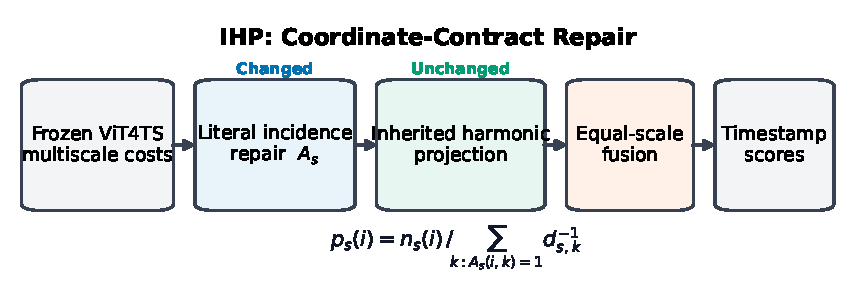
\includegraphics[width=0.98\textwidth]{figures/ihp_method.pdf}
  \caption{IHP is a coordinate-contract repair inside the frozen ViT4TS
  screen. Literal incidence repairs the released zero-based support relation;
  the inherited ViT4TS harmonic projector then aggregates the same frozen
  token costs unchanged on that corrected support. The encoder, visual memory,
  matching, scale fusion, and timestamp stitching remain fixed.}
  \label{fig:ihp}
\end{figure*}

The design follows a single causal chain. Section~\ref{sec:coordinate_failure}
defines the coordinate-contract failure. Sections~\ref{sec:literal_lifting}
and~\ref{sec:harmonic_pullback} present the repair and its inherited reducer, and
Section~\ref{sec:system_integration} specifies the frozen-system boundary and
computational properties. IHP has no training objective, learned parameter,
or label-dependent branch.

\subsection{Frozen Screening Interface}

Let a rendered window be encoded on a $g\times g$ base grid, where the frozen
ViT-B/16 configuration gives $g=14$ and $N=g^2=196$ base cells. We index a
base cell by $i\in\Omega=\{0,\ldots,N-1\}$ and use
$s\in\mathcal{S}=\{\mathrm{b},\mathrm{m},\mathrm{l}\}$ for the base, medium,
and large token scales. Their token counts are $K_{\mathrm{b}}=196$,
$K_{\mathrm{m}}=169$, and $K_{\mathrm{l}}=144$, corresponding to the base
grid and the released overlapping $2\times2$ and $3\times3$ pooling layouts.

For window $w$, let $d_{w,s,k}\geq0$ denote the frozen cosine-dissimilarity
cost of token $k$ at scale $s$. IHP does not alter how this cost is obtained:
the line renderer, CLIP weights, multiscale pooling, median memory, and
unrestricted nearest-memory comparison are fixed. For each pooled token, the
released assets also provide a set
$M_{s,k}\subseteq\Omega$ containing the flattened base-cell indices that
contributed to that token. These sets are the sole geometric input to IHP.

\subsection{Failure Mechanism: A Shifted Support Graph}
\label{sec:coordinate_failure}

We call a multiscale projector \emph{index-consistent} when the support used
to score output cell $i$ is exactly the set of tokens whose provided
membership contains $i$. However, the released implementation queries the
already zero-based memberships with a one-step shift. Its effective incidence
matrix is
\begin{equation}
 A^{\mathrm{rel}}_s(i,k)
 =\mathbb{1}\!\left[i+1\in M_{s,k}\right],
 \qquad i\in\Omega ,
 \label{eq:released_incidence}
\end{equation}
where $A^{\mathrm{rel}}_s(i,k)$ indicates whether scale-$s$ token $k$ is used
for output cell $i$, $M_{s,k}$ is the released zero-based membership set, and
$\mathbb{1}[\cdot]$ is the indicator function.

Equation~\eqref{eq:released_incidence} advances every support query by one
flattened cell. At each pooled scale, 195 of 196 queries return valid support,
but all 195 are displaced. Thirteen shifts, at indices
$13,27,\ldots,181$, wrap across a row boundary; the remaining valid queries
move within a row. The terminal output cell $i=195$ queries index 196, which
cannot occur in $M_{s,k}\subseteq\{0,\ldots,195\}$ and therefore has no
pooled-token support. A subsequent finite-value fallback converts this
structural hole into a zero anomaly contribution. The mismatch is thus a
localization failure at the frozen token-to-grid interface rather than a
shortage of encoder capacity.

\subsection{Literal Incidence Repair}
\label{sec:literal_lifting}

IHP first lifts each provided membership set into a literal incidence matrix:
\begin{equation}
 A_s(i,k)=\mathbb{1}\!\left[i\in M_{s,k}\right],
 \qquad A_s\in\{0,1\}^{N\times K_s}.
 \label{eq:literal_incidence}
\end{equation}
Here, $A_s(i,k)$ links base cell $i$ to pooled token $k$, $N=196$ is the
number of output cells, and $K_s$ is the number of tokens at scale $s$. The
base scale uses the identity incidence $A_{\mathrm{b}}=I_N$ because each base
token already corresponds to one output cell.

Literal lifting is needed because a flattened index has meaning only under
the coordinate convention that generated it. Equation~\eqref{eq:literal_incidence}
uses the stored convention directly and introduces neither a learned mapping
nor a corrective offset. Consequently, it preserves every supplied
token--cell relation while removing the one-cell displacement, including its
13 row wraps, in Eq.~\eqref{eq:released_incidence}.

\noindent\textbf{Complete-coverage property.}
Let $n_s(i)=\sum_{k=1}^{K_s}A_s(i,k)$ be the number of scale-$s$ tokens
incident to cell $i$. If the released pooling layout covers the base grid,
$\bigcup_{k=1}^{K_s}M_{s,k}=\Omega$, then
$n_s(i)\geq1$ for every $i\in\Omega$. This follows directly because each
covered index appears in at least one membership set. The supplied medium and
large masks satisfy this premise, so literal lifting produces valid support
for all 196 cells without interpolation or an artificial terminal value.

\subsection{Inherited Harmonic Projection on Corrected Support}
\label{sec:harmonic_pullback}

After support is restored, IHP pulls each pooled token cost back to every base
cell that contributed to it. For a pooled scale
$s\in\{\mathrm{m},\mathrm{l}\}$, let
$\mathcal{I}_s(i)=\{k:A_s(i,k)=1\}$ denote the incident token set. The
projected cost is
\begin{equation}
 p_{w,s}(i)=
 \begin{cases}
 0, & \min_{k\in\mathcal{I}_s(i)}d_{w,s,k}=0,\\[2pt]
 \displaystyle
 \frac{n_s(i)}{\sum_{k\in\mathcal{I}_s(i)}d_{w,s,k}^{-1}},
 & \text{otherwise}.
 \end{cases}
 \label{eq:harmonic_pullback}
\end{equation}
In Eq.~\eqref{eq:harmonic_pullback}, $p_{w,s}(i)$ is the scale-$s$ cost at
base cell $i$ for window $w$, $d_{w,s,k}$ is the frozen nonnegative token
cost, $\mathcal{I}_s(i)$ is the literal incident set, and $n_s(i)$ normalizes
for the number of incident tokens. The first branch is the exact zero convention used
by the implementation: an incident zero dissimilarity makes the harmonic
cost zero, so no numerical $\epsilon$ or tunable floor is introduced.

The harmonic reducer and its support normalization are inherited from
ViT4TS; IHP does not claim a new mean in isolation. Its evaluated output is
different from the released path because the unchanged reducer is composed
with the index-consistent support graph and is defined for every output cell.
The normalization prevents cells covered by more overlapping pooled tokens
from receiving a larger value merely because their support cardinality is
larger.

The three frozen scales are fused with the released equal-scale average,
\begin{equation}
 P_w(i)=\frac{1}{3}\left(
 d_{w,\mathrm{b},i}+p_{w,\mathrm{m}}(i)+p_{w,\mathrm{l}}(i)
 \right),
 \label{eq:scale_fusion}
\end{equation}
where $P_w(i)$ is the final base-grid cost for window $w$,
$d_{w,\mathrm{b},i}$ is the base-token cost at cell $i$, and the remaining
terms are the medium- and large-scale pullbacks from
Eq.~\eqref{eq:harmonic_pullback}. Thus, no scale weight is learned or selected
per dataset.

\subsection{Frozen-System Integration and Properties}
\label{sec:system_integration}

The vector $P_w\in\mathbb{R}^{196}$ is reshaped to $14\times14$, bilinearly
upsampled to $224\times224$, reduced with the released top-quarter column
mean, and stitched across overlapping windows using the released temporal
alignment. These operations, the anomaly threshold sweep, and the optional
downstream VLM verification are outside IHP and remain unchanged. The present
system evaluates the frozen visual screening stage; it does not attribute
language-model reasoning to IHP.

IHP is deterministic, training-free, and parameter-free. Constructing the
fixed incidence matrices and applying Eq.~\eqref{eq:harmonic_pullback} has the
same asymptotic projection complexity as the released membership queries.
Most importantly, IHP reuses the same rendered windows, frozen visual tokens,
memory, and token costs, so it adds no encoder forward pass. Test labels are
read only by the evaluator after complete score files have been committed;
they do not enter incidence construction, projection, fusion, or stitching.

\section{Experimental Protocol}

The experiment uses the fixed TSB-AD evaluation lists~\cite{liu2024elephant}
and threshold-free VUS-PR as its primary endpoint~\cite{paparrizos2022vus}.
ResearchPilot G.2 will insert the exact frozen arms, environment, aggregation,
and failure disclosures from compact artifacts only.

\section{Results and Analysis}
\label{sec:results}

\subsection{Same-Cache Projection Ablation}

Table~\ref{tab:ablation} is the primary causal comparison. Relative to
\textsc{REL-U}, IHP raises equal-subdataset F1-max from 0.6354 to 0.6621,
AUPRC from 0.2974 to 0.3192, and VUS-PR from 0.6873 to 0.6975. The observed
differences are +0.0267, +0.0218, and +0.0102. The unadjusted intervals
exclude zero for AUPRC and VUS-PR, while the F1-max interval extends to
-0.0023. These intervals describe sampling variability under the paired
benchmark hierarchy and are not adjusted for the component-arm selection
disclosed in Section~\ref{sec:experiments}.

\begin{table}[t]
  \centering
  \caption{Same-cache projection ablation on 492 paired series. Intervals use
  10,000 hierarchical bootstrap replicates and are unadjusted for arm
  selection. ``Positive'' counts subdatasets with a positive IHP-minus-
  \textsc{REL-U} difference.}
  \label{tab:ablation}
  \footnotesize
  \resizebox{\columnwidth}{!}{%
  \begin{tabular}{lrrrrr}
    \toprule
    Metric & \textsc{REL-U} & IHP & $\Delta$ & 95\% interval & Positive \\
    \midrule
    F1-max & .6354 & .6621 & +.0267 & [-.0023, .0681] & 6/11 \\
    AUPRC  & .2974 & .3192 & +.0218 & [.0062, .0398] & 9/11 \\
    VUS-PR & .6873 & .6975 & +.0102 & [.0021, .0197] & 7/11 \\
    \bottomrule
  \end{tabular}%
  }
\end{table}

The subdataset distribution shows that the ranking gains are not confined to
one family. IHP improves AUPRC on 9/11 groups, with its largest gains on
Yahoo-A1 (+0.0768) and Yahoo-A2 (+0.0584); the largest AUPRC loss is -0.0116
on NAB-Tweets. VUS-PR gains most on Yahoo-A1 (+0.0367) and Yahoo-A2
(+0.0360), whereas its largest loss is -0.0053 on NASA-SMAP. F1-max is more
heterogeneous: IHP gains +0.1680 on NAB-Artificial and +0.0913 on NAB-Traffic
but loses -0.0174 on NASA-SMAP. This heterogeneity is consistent with the
wider F1-max interval and its arm-specific maximizing operating point.

\begin{figure*}[t]
  \centering
  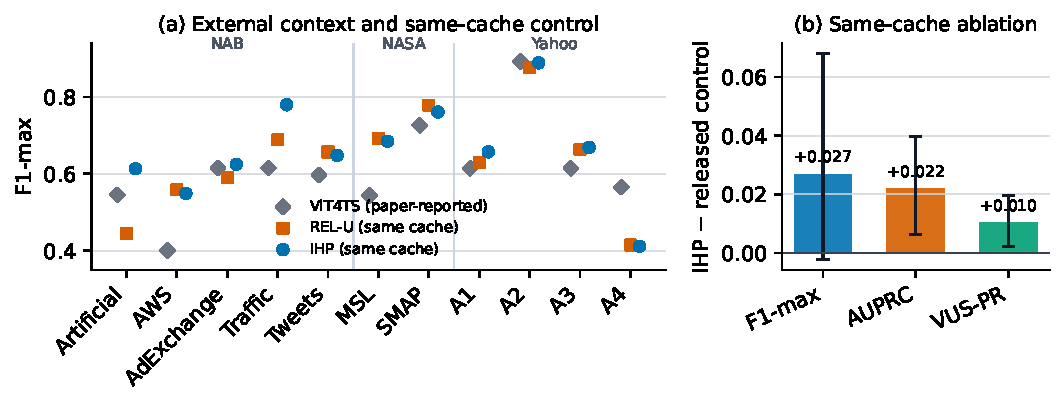
\includegraphics[width=0.97\textwidth]{figures/ihp_results.pdf}
  \caption{Full evidence summary. (a) External paper-reported ViT4TS and the
  two local same-cache F1-max arms across eleven categorical subdatasets; the
  markers are intentionally unconnected. (b) Same-cache IHP-minus-
  \textsc{REL-U} differences with unadjusted hierarchical 95\% intervals.
  The F1-max interval crosses zero; the AUPRC and VUS-PR intervals do not.}
  \label{fig:results}
\end{figure*}

\subsection{External Paper-Reported Context}

Table~\ref{tab:external} separates the paper-reported ViT4TS values from the
two local same-cache arms. IHP obtains equal-subdataset F1-max 0.662 versus
the external ViT4TS value 0.612 and is numerically higher on 9/11
subdatasets. However, the local released-coordinate control already obtains
0.635; consequently, the external +0.050 difference is not the IHP effect.
The attributable local difference is the paired +0.027 reported above.

\begin{table}[t]
  \centering
  \caption{Complete F1-max context for the VLM4TS Table~1 taxonomy.
  ViT4TS$^{\mathrm{P}}$ is external and paper-reported; \textsc{REL-U}, IHP,
  and $\Delta_{\mathrm{pair}}$ are local same-cache results. Cross-environment
  columns are not a paired ranking.}
  \label{tab:external}
  \footnotesize
  \setlength{\tabcolsep}{2.3pt}
  \resizebox{\columnwidth}{!}{%
  \begin{tabular}{lrrrrr}
    \toprule
    Subdataset & $n$ & ViT4TS$^{\mathrm{P}}$ & \textsc{REL-U} & IHP & $\Delta_{\mathrm{pair}}$ \\
    \midrule
    NAB-Artificial & 6   & .545 & .445 & .613 & +.168 \\
    NAB-AWS        & 17  & .400 & .558 & .549 & -.009 \\
    NAB-AdExchange & 5   & .615 & .590 & .624 & +.034 \\
    NAB-Traffic    & 7   & .615 & .688 & .779 & +.091 \\
    NAB-Tweets     & 10  & .597 & .656 & .648 & -.009 \\
    NASA-MSL       & 27  & .543 & .692 & .684 & -.008 \\
    NASA-SMAP      & 53  & .726 & .778 & .760 & -.017 \\
    Yahoo-A1       & 67  & .614 & .628 & .657 & +.029 \\
    Yahoo-A2       & 100 & .892 & .876 & .888 & +.013 \\
    Yahoo-A3       & 100 & .614 & .663 & .669 & +.005 \\
    Yahoo-A4       & 100 & .565 & .415 & .411 & -.003 \\
    \midrule
    Equal-11       & 492 & .612 & .635 & .662 & +.027 \\
    \bottomrule
  \end{tabular}%
  }
\end{table}

The full paper-reported VLM4TS system reaches 0.659, but it adds an external
language-model verification stage absent from both local arms. We therefore
do not use it as a paired comparator. Yahoo-A4 further illustrates the
environment boundary: IHP is 0.154 below the external ViT4TS entry but only
0.003 below the local control, while its same-cache AUPRC and VUS-PR increase
by 0.0157 and 0.0069. This discrepancy is compatible with threshold and
environment differences and prevents a causal reading of the external rows.

\subsection{Structural Certificate and Computational Boundary}

Table~\ref{tab:certificate} tests the mechanism without labels. At both
pooled scales, every one of the 195 released queries that finds support is
shifted by one flattened cell. Thirteen of those shifts wrap across row
boundaries, and the terminal query is unsupported. Literal incidence covers
all 196 output cells. The medium and large mask hashes are identical across
all 492 cached transactions, so the certificate is not inferred from a
single selected series.

\begin{table}[t]
  \centering
  \caption{Label-free support-graph certificate on the $14\times14$ grid.
  ``Rel. valid'' counts shifted queries returning support; all 195 are
  displaced. ``Row wraps'' is the subset crossing a row boundary.}
  \label{tab:certificate}
  \footnotesize
  \resizebox{\columnwidth}{!}{%
  \begin{tabular}{lrrrrr}
    \toprule
    Scale & Output & Rel. valid & IHP valid & Row wraps & Holes \\
    \midrule
    Medium & 196 & 195 & 196 & 13 & 1 \\
    Large  & 196 & 195 & 196 & 13 & 1 \\
    \bottomrule
  \end{tabular}
  }
\end{table}

IHP introduces zero trainable parameters, consumes no labels, and reuses the
same CLIP token cache. All 492 paired manifests agree in cache key, token hash,
cache-manifest hash, and encoder-call count. Replacing \textsc{REL-U} with IHP
therefore adds zero token-cache bytes and preserves the persisted score
footprint (11.82~MiB for all 492 series). It also adds no encoder pass or
external-VLM call; only the fixed incidence lookup changes before the
inherited harmonic reduction. Runtime and peak allocated VRAM were recorded
jointly for three experimental arms, so we make no arm-isolated latency, VRAM,
or host-RAM claim. The exact certificate and paired threshold-free
improvements support the narrower conclusion that the projection interface,
rather than additional model capacity, changes the anomaly ranking.

\section{Limitations and Conclusion}

This work audited whether a frozen visual anomaly screen returns multiscale
evidence to the base-grid cells that generated it. The released ViT4TS
projector shifts every valid pooled-scale query by one flattened cell and
leaves the terminal query unsupported. IHP provides the minimal repair: it
uses the supplied zero-based memberships literally and then applies the
unchanged harmonic projector on the corrected support. In the 492-series
same-cache comparison, IHP improves equal-subdataset F1-max, AUPRC, and VUS-PR
by 0.0267, 0.0218, and 0.0102. Unadjusted intervals exclude zero for AUPRC
and VUS-PR but not F1-max. The paper-reported ViT4TS value of 0.612 and IHP's
0.662 provide secondary external context, not a paired method effect.

The evidence is bounded to the univariate ViT4TS screening stage, its released
$14\times14$ grid and pooling masks, and three benchmark families. IHP was a
prespecified component promoted after a composite candidate failed on the same
evaluation, so its intervals are not selection-adjusted. Moreover, released
full-series preprocessing and all-window median memory make the evaluated
screen offline and transductive; IHP does not remove this deployment
limitation. We do not evaluate downstream VLM verification, multivariate
renderers, online drift, or other visual backbones. Future work should make
coordinate contracts executable across other renderers and test them on an
independent, streaming-compatible protocol. Within the present boundary, the
exact 196/196 coverage certificate and paired ranking gains show that auditing
an inverse-coordinate interface can improve a frozen screen without training,
labels, learned parameters, or another encoder pass.


\bibliographystyle{IEEEtran}
\bibliography{references}

\end{document}
